\documentclass[12pt]{report}
\usepackage[utf8]{inputenc}
\usepackage{graphicx}
\usepackage{float}
\graphicspath{ {images/} }
\counterwithout{figure}{chapter}
\counterwithout{table}{chapter}
\renewcommand{\bibname}{References}
\usepackage{array}
\usepackage{varwidth}

\begin{document}
\newcolumntype{M}{>{\begin{varwidth}{10cm}}l<{\end{varwidth}}}
\newcolumntype{S}{>{\begin{varwidth}{8cm}}l<{\end{varwidth}}}


\title{
{Topic Modelling for Emerging Risk Identification from Company Annual Financial Reports}\\
{\large University Of Manchester}\\
{\large Department Of Computer Science}\\}
\author{By Zygimantas Koncius\\Supervised By Goran Nenadic}
\date{April 2020}
\maketitle

\chapter*{Abstract}
Company annual financial reports are a very useful source of information about company's performance, opportunities and risks in the industries. Considering the amount of data contained in every report and amount of reports from different companies available, there is a strong motivation to automate processing of this information, this way gaining more insights into the current state of industries.
\\\\
The project described in this report is aimed to create a method that is able to automatically identify emerging risks faced by multiple businesses and the trends of those risks. The research focuses on first story detection, classification and topic modelling in annual financial reports. The features used for these approaches were based on a sentence level granularity. In the final design of the method, one of the core components was classifying each of the sentences into 1 of 30 known constant risks or keeping it unclassified. After classification, the topics were generated from the unclassified sentences using Latent Dirichlet Allocation (LDA). This method has been tested on a dataset containing 53,093 SEC 10-K filings. The outcome of it was between 30 and 50 topics for the whole dataset and 10 topics for every year in the dataset.
\\\\
Extracting the most useful information from the textual financial report data and correctly interpreting it is an ongoing challenge and hopefully methods used in this project will prove to be useful in future research.

\chapter*{Acknowledgements}
I would like to express my gratitude to my supervisor, Dr Goran Nenadic for
his guidance, support and suggestions throughout the whole project.\\\\
I would also like to thank Dr Stefan Petry from Alliance Manchester Business
School for sharing materials relevant to the project as well as passing some of his knowledge in the field of business and helping throughout the course of the project.

\tableofcontents
\listoffigures
\listoftables

\chapter{Context}

\section{Motivation}
This project focuses on U.S. company annual report 10-K forms required by U.S. Securities and Exchange Commission (SEC). These forms are lengthy ($\sim$100 pages long) documents, that have to comply with SEC requirements. These forms are an important source of information for company's stakeholders, about the business' business performance, future plans as well as risks that company has to face.

The main focus of the project are the emergence of the risks. Which are conveniently represented by a separate section in 10-K forms. Risks play an  important role in predicting the future of the businesses or even the whole industries. The risks can be categorized into known, constant risks - the risks that are reoccuring every year, such as \textit{catastrophes, financial liability and financing uncertainty} - and emerging risks - the risks that are novel and possibly unseen before, such as \textit{cybersecurity or COVID-19}. The main focus of this project is on the detection of the latter.

Due to the number of companies and reports (between 3000 and 5000 of $\sim$100 page long reports every year) it is impossible for any person to analyze all of them. Therefore, an automatic risk emergence detection could offer unprecedented insights into the industries as a whole, as it would be possible to proccess much more documents than any human could ever read.

Furthermore, identifying risk trends early could provide a significant competitive advantage to the investors, who could make insightful, data-backed investment decisions, before others, providing them with the capability to make better investments.

\section{Aim}
The aim of this project is creating a system which - given the set of financial reports - is capable of automatically identifying emerging, before unseen risks.

\section{Objectives}
In order to achieve the aim of the project, the following objectives have been set:
\begin{itemize}
\item Analyse the dataset, document structure and preprocess the data
\item Extract the risk sections
\item Develop a method to identify known type of risks
\item Identify emerging risks, potentially by using topic modelling
\item Analyse and evaluate the results
\end{itemize}

\section{Outcomes}
The project resulted in following outcomes:
\begin{itemize}
\item A method to parse the annual financial reports and extract risk sections from them
\item A method to filter out known, constant risks from the dataset
\item A method to identify potential emerging risks
\end{itemize}

\section{Impact of COVID-19}
As this project is purely software-based and all of the required computational resources were not disrupted and accessible at all times, there was no direct impact to the system creation. However, due to the disruptions of communication, planning and cooperation, caused by COVID-19, the evaluation part was difficult to carry out and lacks end user feedback.
\chapter{Background}
\section{Natural Language Processing}
Natural language processing (NLP) is a subfield of linguistics, computer science, information engineering, and artificial intelligence concerned with the interactions between computers and human (natural) languages, in particular how to program computers to process and analyze large amounts of natural language data \cite{nlpdefinition}.

\subsection{NLP Pipeline}
Typical NLP pipelines consist of multiple parts all of which add value to the output and are crucial for any advanced tasks performed on text. Common tasks include tokenization, part of speech tagging, stemming and others.

\begin{figure}[H]
\begin{center}
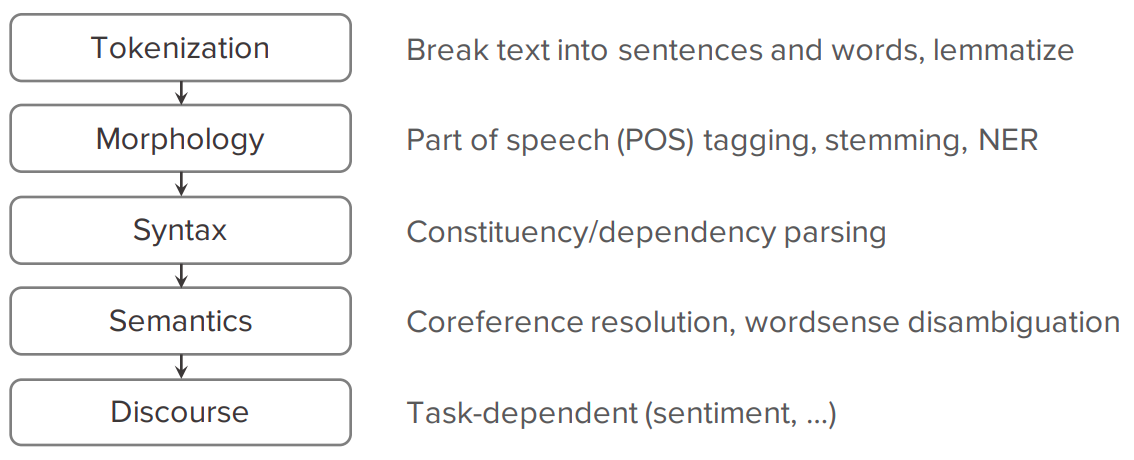
\includegraphics[scale=0.3]{classicalnlppipeline.png}
\caption{Typical NLP pipeline \cite{nlppipeline}}
\end{center}
\end{figure}

\subsubsection{Stopword Removal}
Stopword removal is a common data cleaning technique. Stopwords are common words, which do not provide a lot of value at tackling the task. For example, words such as \textit{and, for, but, on}. Stopwords can be context dependent. Removing stopwords reduces dataset size and lowers the amount of noise in the data, thus improving performance and accuracy of the other pipeline components.

\subsection{Information Retrieval}
Information retrieval is focused on finding documents relevant to the query. While its traditional use cases revolve around search engines it can also be used in other tasks, such as classification. Information retrieval methods are most often based on terms, which can be words or n-grams.

\subsubsection{N-grams}
N-gram is a contiguous sequence of \textit{n} items from a given sample of text or speech \cite{ngramwiki}. The items can be phonemes, syllables, letters or words \cite{ngramwiki}. In this project only word n-grams are going to be used.

\subsubsection{Term Frequency (TF)}
Term frequency assigns weights to words in a set of documents, and it is a count of all of the occurences of a term in a document or a whole dataset. While it is not an accurate weighting method, using it on whole dataset together with n-grams has a potential of providing useful insights into the dataset.
\subsubsection{Inverse Document Frequency (IDF)}
Inverse document frequency is another term weighting method. Document frequency for term \textit{t} shows in how many documents does the term appear. However, it is evident that the most informative and discriminative terms are the ones which occurs in less documents rather than all of them. For example, "spider" is a much more helpful query term than "and". Therefore, inversed document frequency is used.

It is calculated by dividing a total number of documents (\textit{N}) by the number of documents that contain the term (\textit{$df_{t}$}) and then applying the logarithm. The resulting formula is:
\[ idf_{t} = log_{10}(N/df_{t}) \]

\subsubsection{Term Frequency - Inverse Document Frequency (TF-IDF)}
Term Frequency - Inverse Document Frequency (TF-IDF) is very well known and widely used in information retrieval. It is calculated by multiplying term frequency of a term in a specific document ($TF_{i, j}$) with an inverse document frequency of a term in the dataset ($IDF_{i}$):
\[ w_{i,j} = tf_{i,j} * log_{10}(N/df_{t}) \]

\subsubsection{Cosine Similarity}
Cosine similarity is a measure of similarity between vectors, which is often usedn technique in information retrieval. Using cosine similarity it is possible to find documents or sentences that are most similar to the given query. For length-normalized vectors, cosine similarity is a dot product:
\[cos(\vec{a},\vec{b})=\vec{a} \cdot \vec{b}\]
\subsection{Word Embeddings}
Word embeddings are mappings of words or phrases of the vocabulary to vectors of real numbers. One of the biggest breakthroughs in word embeddings has been in 2013 with the creation of Word2vec by Google \cite{wordembeddingwiki}. Since then there have been created a few even more advanced models such as BERT, ELMo and ULMfit, which are contextualixed word embedding models (also called language models) \cite{languagemodels} and are a current state-of-the-art.

One of the core advantages of word embeddings are that they can also be pre-trained on a specific dataset, this way improving their performance in the specific context or in specific tasks.
\subsection{Topic Modelling Using LDA}
\label{sec:lda}
Topic modelling is a procedure of extracting topics from documents. There are multiple multiple topic modelling methods available, but one of the most popular ones is latent Dirichlet allocation (LDA).

LDA is an unsupervised machine learning algorithm, as it does not use labeled data, but generates topics based on statistics \cite{ldawiki}. LDA treats every document as a bag-of-words (i.e. order does not matter) and the key assumption is that the way the document was generated was by picking a set of topics and then for each topic a set of words \cite{ldaexplanation}. And then it basically reverse engineers the process by the following algorithm:
\begin{enumerate}
\item Assume there are \textit{k} topics across the all of the provided documents.
\item Distribute these \textit{k} topics across document \textit{m} (this distribution is known as $\alpha$) by assigning each word a topic.
\item For each word \textit{w} in document \textit{m}, assume its topic is wrong but every other word is assigned the correct topic.
\item Probabilistically assign word \textit{w} a topic based on what topics are in document \textit{m} and how many times word \textit{w} has been assigned a particular topic across all of the documents (this distribution is called $\beta$).
\end{enumerate}

\begin{figure}[H]
\begin{center}
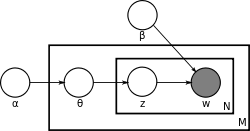
\includegraphics[scale=1.3]{LDAplate.png}
\caption{LDA model plate diagram \cite{riskpaper1}}
\end{center}
\end{figure}

The following are explanations of notation found in the figure and LDA algorithm explanation:
\begin{itemize}
\item $\alpha$ is the per-document topic distributions parameter (a high
$\alpha$ indicates that each document is a mixture of most of the topics, while a low $\alpha$ suggests that the document contains a mixture of just a few of the topics)
\item $\beta$ is the per-topic word distribution parameter (a high $\beta$ indicates that each topic will contain a mixture of most of the words, a low $\beta$ indicated that a topic will contain a mixture of just a few of the words)
\item $\theta$ is the topic distribution for document \textit{m}
\item \textit{z} is the topic for the \textit{n}-th word in document \textit{m}
\item \textit{w} is the specific word
\end{itemize}

\section{Clustering}
Clustering is the task of grouping a set of objects in such a way that objects in the same group (called a cluster) are more similar (in some sense) to each other than to those in other groups (cluster) \cite{clusteringWiki}. Clustering is considered an unsupervised machine learning method, which helps provide insights into data by automatically clustering it.

\subsection{K-means clustering}
The K-means clustering algorithm is an iterative algorithm that tries to partition the dataset into \textit{K} pre-defined distinct non-overlapping groups (clusters). It tries to make the inter-cluster data points as similar as possible while also keeping the clusters as different as possible. It assigns data points to a cluster such that the sum of the squared distance between the data points and the cluster’s centroid is at the minimum \cite{kmeansexplanation}. K-means is implicitly based on Euclidean distances. K-means clustering works well, when the cluster number is known.

\subsection{Density-based spatial clustering of applications with noise (DBSCAN)}
Density-based spatial clustering of applications with noise (DBSCAN) \cite{dbscanwiki} is another clustering algorithm, which does not need a pre-defined number of clusters and instead it automatically clusters data points into dense regions and filters out noise. Therefore uses parameters: 
\begin{itemize}
\item \textit{MinPts} - specifies what is the smallest acceptable size of the cluster (smaller clusters are treated as noise)
\item $\varepsilon$ - a minimum distance used to assign data point to the cluster
\item Distance function - the type of function that calculates the distance between points (for example euclidean or cosine distance function). This choice is tightly coupled with $\varepsilon$ choice.
\end{itemize}

\section{SEC 10-K Form}
The project dataset consists of U.S. Securities and Exchange Commission (SEC) Form 10-K filings, one of the most important sources of corporate information which U.S. corporations are obligated by law to create.

The dataset consists of 53,093 reports from different companies over a 10 year period from 2005 up until 2015.

\begin{table}[H]
\centering
\begin{tabular}{|c|c|}
\hline
Year & Number of Reports \\
\hline
2005 & 4834\\\hline
2006 & 5207\\\hline
2007 & 5192\\\hline
2008 & 5277\\\hline
2009 & 5103\\\hline
2010 & 4980\\\hline
2011 & 4835\\\hline
2012 & 4735\\\hline
2013 & 4754\\\hline
2014 & 4712\\\hline
2015 & 3464\\\hline
\end{tabular}
\caption{Dataset Distribution}
\label{table:1}
\end{table}

The documents are .txt files in which there is a specific SEC header and then HTML content. The reports are typically up to 100 pages long and follow a similar structure, consisting of 15 items organised in four parts:

\begin{figure}[H]
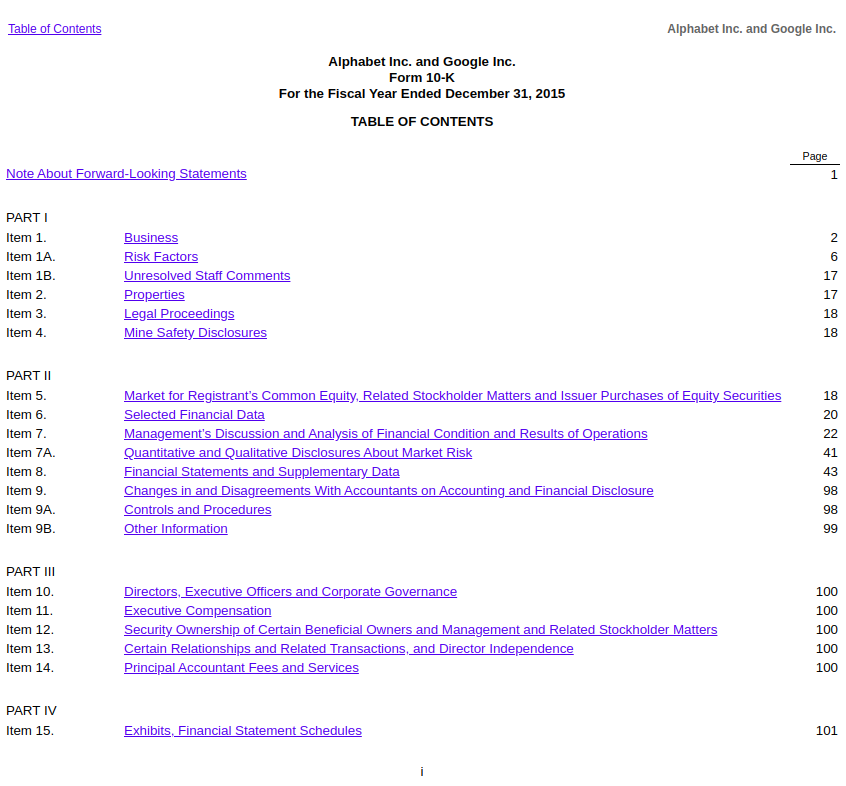
\includegraphics[scale=0.5]{toc.png}
\caption{SEC 10-K filing Table of Contents}
\end{figure}

As the project focuses on risks the only relevant section for it is assumed to be "Item 1A. Risk Factors" in which the risks and threats faced by business are discussed as well as the approaches to mitigating those risks.

\section{Related Research}
Emerging risk detection from SEC 10-K filings is not a well researched topic, however there exists some research on modelling constant, most common, reoccuring risks.

The most relevant and similar research has been done by Yang Bao and Anindya Datta (2012) \cite{riskpaper1}. They have built an algorithm based on latent Dirichlet allocation, which identifies the set of most common topics across the provided financial reports.

Most of previous work has been focused on tackling the risk detection task by using supervised methods, which proved to be fairly inefficient and unscalable. In this research, they built an unsupervised model based on latent Dirichlet allocation (LDA). 

The original LDA operates at the level of the words. However, as in the financial reports in most cases one sentence represents one risk topic, there may occur overlaps of topics in the sentences in case of original LDA. Therefore, they have developed sent-LDA, which tackles this problem by introducing sentence level calculations.

\begin{figure}[H]
\begin{center}
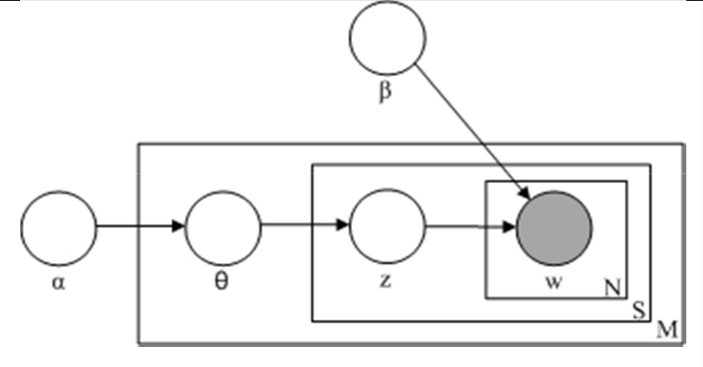
\includegraphics[scale=0.55]{sentLDA.png}
\caption{sent-LDA model representation \cite{riskpaper1}}
\end{center}
\end{figure}

The same notations are used as in original LDA (described in Section \ref{sec:lda}), introducing S as a sentence in a document. The model is created using the generative process (Figure \ref{fig:sentLDAgen}):

\begin{figure}[H]
\center
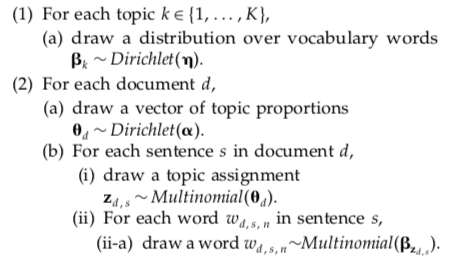
\includegraphics[scale=0.6]{sentLDApseudocode.png}
\caption{sent-LDA generative process \cite{riskpaper1}}
\label{fig:sentLDAgen}
\end{figure}

The described research has been a helpful starting point, which helped me understand the risk topic definitions, provided insight into constant reoccuring risks and helped define this projects approach to the task.
\\\\
Another research related to the project was done by S. Sehrawat \cite{10kwordembeddings}. In which he pre-trained word embeddings on SEC 10-K filings. The result of it was a 300-dimensional word embedding representation model.

\section{Constant Risks}
In this project the risks are categorized into known, constant risks - the risks that are reoccuring every year, such as \textit{catastrophes, financial liability and financing uncertainty} - and emerging risks - the risks that are novel and possibly unseen before, such as \textit{cybersecurity or COVID-19}. The constant risks are represented by a topic model, consisting of keywords and their frequencies. Risk topics are illustrated well by Yang Bao and Anindya Datta (2012) \cite{riskpaper1}:

\begin{figure}[H]
\center
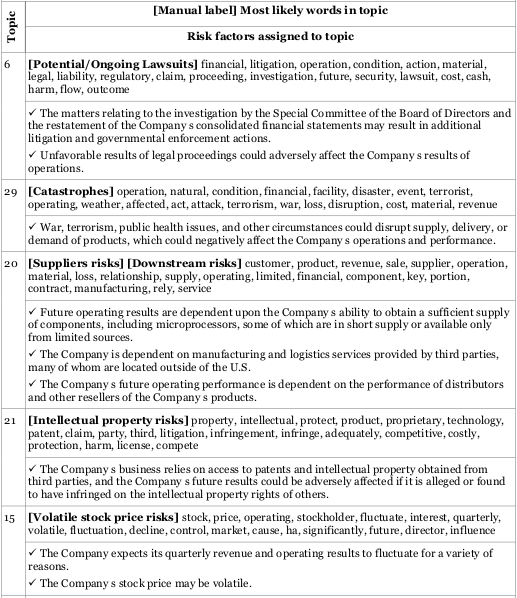
\includegraphics[scale=0.8]{risktopicfromriskpaper1.png}
\caption{Risk topic model example \cite{riskpaper1}}
\end{figure}

The constant risks and their topic model used in this project were generated in a research done by Dr. Stefan Petry\footnote{At the time of the writing the research is still ongoing, therefore the topics and their models cannot be publicly shared.}. The constant risk topic model contains 30 topics (constant risks), each defined by 30 keywords and their frequencies.
\chapter{System Development}
In order to achieve the goal of this project, the workflow and whole system architecture was carefully planned from the very beginning. To achieve high quality results, every part of the system had to produce satisfactory artifacts. Therefore, the system is made of independent parts, all of which have been separately implemented, tweaked and evaluated. Furthermore, as first story and risk emergence detection in financial domain had not been widely researched yet, there has been a lot of experimentation involved.

The goal of this project was to identify the emerging risks. Therefore, firstly the known, constant risks were filtered out (sentences representing them). Then, the remaining sentences were grouped and processed in a way that extracts the emerging risks.

\section{Requirements}
\begin{enumerate}
\item Acquire and organise the large dataset and its metadata.
\item Remove all non-textual data from the documents.
\item Isolate and extract risk factor sections from reports.
\item Perform any optional data cleaning processes.
\item Analyse the dataset using word and n-gram term frequencies and TF-IDF.
\item Classify sentences into one of constant known risks or keep it in remaining emerging risk class.
\item Group remaining risk class sentences by their similarity and/or report release year.
\item Apply LDA model on different groupings in order to extract topics.
\item Analyse the final results.
\end{enumerate}

\section{System Architecture}
\begin{figure}[H]
\begin{center}
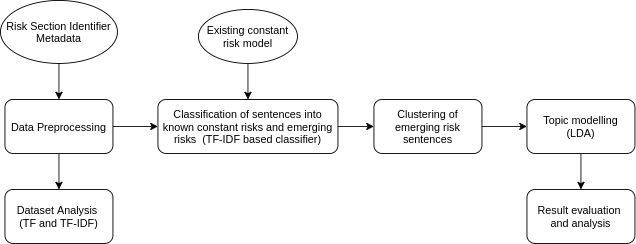
\includegraphics[scale=0.6]{projectArchitecture.png}
\label{fig:architecture}
\caption{System Architecture Diagram}
\end{center}
\end{figure}

This system architecture diagram provides a high-level overview of the system design for this project. Every part of the pipeline, while not fully decoupled is mostly independent and takes in the output of the previous part, as well as some additional data if needed (ellipse parts).

Such architecture provides a capability to tweak, evaluate and reimplement different parts of the pipeline independently as long as the output follows the same format and logic. This is a crucial feature for such project, as major improvements can be made iteratively after gathering and evaluating the end results.

The system was implemented using Python and some common python libraries such as nltk \cite{nltkhome}, scikit-learn \cite{sklearnhome} and others.

\section{Data Preprocessing}
Preparing the dataset is important to achieve high-quality results. While it may seem as a trivial and easy task it proved to be fairly complex, because of inconsistent layout, HTML, structure of reports and the size of the dataset. Therefore, data preprocessing has been divided into three main tasks:
\begin{itemize}
\item parsing the documents into text
\item extracting risk factor sections
\item data cleaning, normalisation
\end{itemize}

\subsection{Document Parsing}
The first step in data preprocessing pipeline was parsing HTML and removing any non-textual elements, keeping only the textual information from the document. This was achieved by using lxml library's HTML parser in Python \cite{lxmlhtml}.

The initial parsing was long and challenging task, which required special handling, because the dataset size was over 600GB. Parsing has reduced the dataset size from $\sim$600GB to $\sim$76GB, which made work with dataset more feasible.

\subsection{Risk Section Extraction}
As this project is focused on working with risks, it was decided to focus only on risk section in the document, which is most often called "Item 1A. Risk Factors". However it is not always clearly and consistently titled section. Fortunately, Dr. Stefan Petry has provided some metadata which includes identifiers of section start and section end sentences. This data came in handy, but it was still not enough in some cases, therefore some additional processing was done in order to standardize whitespaces and capital letters. Furthermore, as often there were more than one matches of those start and end sentences, some additional algorithmic logic was added.

The simple algorithm first finds every start and end sentence occurence and then it chooses such combination, that it is the longest text extract, not having any start or end sentence occurences in it. This way, it was ensured that detected sentences were in fact referring to the section start and end rather than table of content entries or references from other parts of the document.

Furthermore, to filter out outliar risk sections and various risk extraction errors, only the extracts over 1,000 characters and those that were shorter than one-third of the respective report were used. The optimal outliar filtering parameters have been derived by sampling the outliars as well taking into account how many potential risk sections get discarded.

The quality of extraction was verified primarily by random manual sampling, of various length and parameter risk section extracts. However, some additional features were covered by automatic testing of all risk section extracts. One of such features, was checking how many risk section extracts ended with a phrase "unresolved staff comments" as it was fairly common and easily testable parameter, and 35,714 of extracts had that phrase in the end which was a strong suggestion to the correct ending of the extract.

The resulting dataset consisted of 43,795 (out of 53,093 reports) risk sections, amounting to $\sim$2.1GB of data.

\subsection{Normalisation}
Most often for applications dealing with text there are a lot of text normalisation done before. Common examples include case folding, lemmatization and stemming. In this project it was decided that most of those techniques should not be used as a default for all the data due to some of the pipeline steps requiring standard word forms. Therefore, the only normalisation technique applied at data preprocessing step was stopword removal (removing common words with little meaning i.e. and, or, but), stopwords were only left and used at the dataset profiling step.

In some parts of the pipeline further normalisation techniques were used or experimented with (mainly stemming). Also to remove punctuation, word tokenisation was used and punctuation signs were not taken into account in any steps except for dataset profiling.

\section{Dataset Profiling}
Dataset analysis can play an important role at the start of the project, as it provides a better understanding about the project's context. Therefore, in this project term frequency and TF-IDF has been used on words and n-grams to gain some insight into important features of the risk sections.

\subsection{TF}
Term frequency analysis while does not necessarily provide too much insight it can still give some ideas about most common words in the dataset. 

This analysis has been performed on the whole risk section dataset, including stopwords (which can be ignored when analysing). The analysis was run on words with and without using stemming as well as on bi-grams and tri-grams without using stemming. Counting was implemented using Python's Counter while word tokenisation, stemming and n-gram generation was implemented by nltk library \cite{nltkhome}.

\begin{table}[H]
\centering
\begin{tabular}{|l|c|}
\hline
Word & Count \\
\hline
may & 384,301\\\hline
could & 329,270\\\hline
busi & 244,587\\\hline
financi & 214,073\\\hline
result & 287,312\\\hline
risk & 134,397\\\hline
regul & 96,869\\\hline
cyber & 2,031\\\hline
agricultur & 2,017\\\hline
aviat & 1,088\\\hline
\end{tabular}
\caption{Random Stemmed Word Term Frequency Extract}
\label{table:tfstem}
\end{table}

\begin{table}[H]
\centering
\begin{tabular}{|l|c|}
\hline
N-gram & Count \\
\hline
results of operations & 81,660\\\hline
financial condition & 71,326\\\hline
adversely affect & 67,969\\\hline
material adverse effect & 36,237\\\hline
december 31 & 26,049\\\hline
rules and regulations & 2,617\\\hline
cyber attacks & 522\\\hline
\end{tabular}
\caption{Random (2,3)-gram Term Frequency Extract}
\label{table:tfngrams}
\end{table}

The data extracts can provide a few important insights:
\begin{itemize}
\item A lot of speculative, future oriented language ('may', 'could', 'would')
\item A lot of common business performances terms ('result', 'financial')
\item Negatvie sentiment can be found ('adeversely affect', 'risk')
\item Constant risks can be found ('financi', 'regul', 'rules and regulations')
\item Newly, less popular risks can be found when looking at less frequent terms ('cyber', 'cyber attacks', 'aviat', 'agricult')
\item Importance of 31st December, end of the year in the context of the reports.
\end{itemize} 

\subsection{TF-IDF}
Term frequency - inverse document frequency analysis is another useful early stage analysis tool. While usually TF-IDF would be used on document basis, calculating it on whole dataset, it can provide insights into important keywords in the dataset, potentially, uncovering some early clues about the risks that can be found in the dataset.

Because usually TF-IDF would be calculated on document basis, most libraries are implementing it that way, therefore a custom implementation of TF-IDF was built. Using TFIDFVectorizer from scikit-learn package \cite{sklearnhome} inverse document frequencies were extracted, then all that was left to do was combined inverse document frequencies with previously calculated term frequencies (term frequencies of the whole dataset).

This custom TF-IDF calculation was run on the same dataset and its preprocessing variants as term frequency analysis (stemmed word, non-stemmed words, bi-grams, tri-grams).

\begin{table}[H]
\centering
\begin{tabular}{|l|c|}
\hline
Term & TF-IDF \\
\hline
loans & 34701.2115769626\\\hline
nuclear & 27130.4207448989\\\hline
decommissioning & 16524.391082016\\\hline
intellectual property & 14121.7057905634\\\hline
oil and gas & 13950.7980818019\\\hline
the merger & 11483.1921567622\\\hline
information technology & 7674.83078275194\\\hline
credit risk & 6943.80076762693\\\hline
information technology systems & 5413.98271394986\\\hline
cyber & 4166.54304462543\\\hline
cyber security & 1517.5070726361\\\hline
\end{tabular}
\caption{Random (1,2,3)-gram TF-IDF Extract}
\label{table:tfidfall}
\end{table}

Table \ref{table:tfidfall} illustrates some of the terms, which have relatively high TF-IDF scores (the scores span from $\sim$100,000 to $\sim$0.5). It can be seen that this method already extracts some potential risk mentions, such as \textit{loans, nuclear field specific risks, decomissioning} and others, as well as lowers the score of some constant common risks such as \textit{credit risk}. However, compared to those risks, emerging risks such as cyber securiy and information technology are still often ranked lower than a lot of constant risks.

\section{Classification of Sentences Into Constant and Emerging Risks}
\label{sec:classification}
During the design phase of the project, it was decided that to achieve insights into less common, newly emergin risks, there was a need to filter out the constant known risks first, leaving only the sentences with potential emerging risks.

\subsection{TF-IDF Based Classification Algorithm}
Due to having only keywords for topics available and not a full ontology, traditional sentence classification models were not feasible in this project as they are mostly trained on labeled sentences. The choices were to either use the provided topic keywords as seed words or to create a TF-IDF based classifier. As TF-IDF based method implementation was much simpler to implement it was a first choice. Furthermore, it was used in a similar context in research in which they used TF-IDF to vectorize sentences and base the classification on cosine similarities\cite{tfidfclassificationresearch}. However there was a major difference in the approach because they used labeled sentences as their training data, which was not feasible in this project.

The custom model was implemented by first generating the vector of the topic, which was done by adding all the keywords to one sentence and vectorizing it using TFIDFVectorizer from scikit-learn package in Python \cite{sklearnhome}. Then every sentence from the dataset, which is longer than 5 words is converted to TFIDF vector as well and for every sentence the nearest topic vector is found by calculating their cosine similarities. Then based on the threshold parameter and the similarity of the sentence to the most similar topic it is either classified as one of 30 constant risks or as a newly emerging risk sentence (unclassified class). After a lot of experimentation this parameter has been set to be 0.05 (meaning, that if similarity $<$0.05 then it is an unclassified emerging risk sentence).

\subsection{Evaluation of Classification}
The result of this classification yielded 11.01\% of all sentences to remain unclassified (i.e. potential emerging risk sentences). The testing of this classification method was based mainly on manual sampling of different similarity score sentences, from such evaluation the accuracy of classified class was extremely high ($\sim$90\%). The sentences that were left unclassified also seemed promising with $\sim$75\% of them having potential to identify emerging risks. However, the evaluation was very subjective as a lot of sentences were ambiguous.

{\renewcommand{\arraystretch}{2}%
\begin{table}[H]
\centering
\begin{tabular}{|S|c|c|}
\hline
Sentence (without stopwords) & Topic label & Similarity \\
\hline
Debt equity capital may continue available us favorable terms, all. & Financing Uncertainty & 0.170663803\\[5pt]\hline
inability obtain financing favorable terms could adversely affect results operations financial condition. & Financing Uncertainty & 0.271898346\\[5pt]\hline
addition, loan agreements contain financial covenants require us comply specified financial ratios tests relating fixed charge coverage minimum working capital tangible net worth levels. & Financial Liability & 0.101999065\\[5pt]\hline
Acquisitions expose us risks, including risk may unable effectively integrate acquisitions. & Real Estate & 0.071584165\\[5pt]\hline
\end{tabular}
\caption{Constant risk sentence examples and their similarity score to the most similar constant risk topic}
\label{table:classifiedclassexample}
\end{table}

From Table \ref{table:classifiedclassexample} it can be seen that categorized sentences are indeed corellating with constant financial risks, such as financing, loans and acquisitions.

\begin{table}[H]
\centering
\begin{tabular}{|Mc|}
\hline
Sentence (without stopwords) &\\
\hline
FAA, airlines others industry heightened sensitivity scrutiny respect compliance approved maintenance procedures.&\\[5pt]\hline
recently, demand air transportation United States abroad decreased due adverse changes deterioration U.S. global economies.&\\[5pt]\hline
example, European Union (EU) China two among growing number jurisdictions enacted recent years restrictions use lead, among chemicals, electronic products countries considering similar restrictions.&\\[5pt]\hline
past year, cyber-attacks become prevalent much harder detect defend against.&\\[5pt]\hline
\end{tabular}
\caption{Uncategorized, potential risk sentences}
\label{table:uncategorizedclassexample}
\end{table}

Table \ref{table:uncategorizedclassexample} shows some of the examples of potential emerging risk sentences, which refer to specific events in the airline industry, specific restrictions to electronic products and finally cyber attacks.

\section{Clustering Emerging Risk Sentences}
Even after filtering out constant risk sentences, there were still many sentences left that were repeated in the same documents year after year. Therefore, it was decided to try to organise them by similarity and this way have the first unique occurence of the sentence and therefore the first occurences of potential risks.

\subsection{Word Embedding Representation}
\label{sec:wordembeddingsentenceuse}
For word and sentence representation, word embeddings were chosen as they are a good modern and fairly universal technique used for text processing tasks. Furthermore, they can be pre-trained on the dataset to work in the specific context and that has been previously done on this specific dataset. 

The pre-trained financial word embedding model \cite{10kwordembeddings} was imported, then every sentence was converted into a bag-of-words, then every word was using the word embeddings translated to vector and these from these vectors the mean average was calculated which was the representation of the sentence.

\subsection{K-Means Clustering}
First consideration was using one of the most standard clustering algorithms, K-Means clustering. However there was a major drawback with it as it had to have pre-set number of clusters. That meant that there was no good way to cluster sentences into clusters with assured first occurences.

However, it was still tried out in an attempt to use it as a topic modelling tool, which would represent the topic by its center. However that attempt failed, because most of the cluster centres were not represented by sentences and the results were impossible to convert back to textual form.

One other limitation discovered in various experimentations with K-means was that it is using Euclidean distance and changing this into cosine distance instead requires converting k-means algorithm into spherical k-means.

\subsection{Density-Based Spatial Clustering of Applications with Noise (DBSCAN)}
\label{sec:dbscanclusters}
DBSCAN is much less common clustering algorithm. However it has a very important advantage of not needing to set the number of clusters, but providing the maximum distance ($\varepsilon$) to put data points into cluster instead and minimum size of the cluster. Such behaviour makes it perfect for clustering sentences into clusters of similar meaning and finding the first mentions. Furthermore, its implementation enables an easy choice of distance metric. Therefore cosine distances can be easily used instead of Euclidean distance. Finally, it also filters out the "noise", which in this case are the sentences that do not reappear in a similar form in documents.

The DBSCAN in this projected was implemented using scikit-learn package \cite{sklearnhome} and passing the sentence vectors created from word embeddings (as described in Section \ref{sec:wordembeddingsentenceuse}). The $\varepsilon$ through experimentation was chosen to be 0.1 and minimum cluster size was chosen to be 2. The clustering algorithm processed 1,191,452 potentially emerging risk topic sentences, 142,897 of which were considered to be "noise"(not reoccuring) and the rest were clustered into 156,930 clusters.

\begin{table}[H]
\centering
\begin{tabular}{|Mc|}
\hline
Sentence (without stopwords) &\\
\hline
Many files digitized employees working almost paperless environments.&\\[5pt]\hline
Many Company's files digitized employees working almost paperless remote environments.&\\[5pt]\hline
Many files digitized employees working almost paperless environments.&\\[5pt]\hline
Many Company's files digitized employees working almost paperless remote environments.&\\[5pt]\hline
Many files digitized employees working almost paperless environments.&\\[5pt]\hline
\end{tabular}
\caption{Single DBSCAN Cluster Example}
\label{table:dbscanclusterexample}
\end{table}

Table \ref{table:dbscanclusterexample} illustrates the similarity level among the sentences clustered into the same cluster. This example correlates with most clusters, in which the sentences are very similar among themselves. Therefore they can be treated as first occurence of particular sentence identifying clusters.

\section{Topic Modelling Using LDA}
Topic modelling was the final step of this project. It is also the part at which the final results can be seen. The topic modelling itself in this project is implemented by using LDA from scikit-learn package \cite{sklearnhome}. However, as there has been a lot of previous steps to prepare the data for topic modelling and only appply it on the part of the dataset that has a potential to contain emerging topics, the topic modelling is applied in three different experiments on the data prepared by previous steps.

\subsection*{Applying LDA on All Potentially Emerging Risk Sentences}
This is the most straightforward approach in which some insights can be gained and possibly new emerging risks identified. As it is fairly big document set, the topic number experimented with was between 30 and 50.

\subsection*{Applying LDA on The First Mentions of Similar Sentences}
By applying LDA only to the first mentions of the potential risk there can be uncovered most important newly emerging risks, which are mentioned in different ways and probably in different documents. Therefore such approach could potentially yield the most diverse set of newly emerging risks. The first mentions of reoccuring sentences were derived from DBSCAN clusters (described in Section \ref{sec:dbscanclusters}) and the year that the sentences were used in (from metadata). Then the LDA was applied on those sentences, by treating every sentence as a separate document. For this approach the number of topics experimented with was between 30 and 50 as well.

\subsection*{Applying LDA Separately For Every Year}
Applying LDA on a subset of data by dividing documents by year can reveal more about the topic distributions every year as well as it can directly show the risk changes throughout time. For this approach, after a lot of experimentation, the number of topics was chosen to be 10 for every year.


\chapter{Results and Evaluation}
The end result of this project were risk topics generated from the potential emerging risk sentences, organized in different ways, this way providing a variety of results for evaluation.

\section{Experiment 1: Full}
The LDA was ran on the dataset consisted of documents with remaining emerging risk sentences, identified as such by the classification part (Section \ref{sec:classification}). The LDA was run with topic parameter set to 30 and 50.

{\renewcommand{\arraystretch}{1}%
\begin{table}[H]
\centering
\resizebox{\columnwidth}{!}{%
\begin{tabular}{|c|l|}
\hline
Topic number & Topic keywords \\\hline
0 & products tests test testing research cancer diagnostic clinical patents cell \\\hline
1 & products patents agreements research parties technologies rights development addition terms \\\hline
2 & solar cms hospitals tissue brazilian products states services facilities regulations \\\hline
3 & products memory storage semiconductor customers flash sales based test design \\\hline
4 & vessels vessel charter rates fleet charters shipping time addition market \\\hline
5 & products customers sales services systems solutions competitors technologies business addition \\\hline
6 & advertising 000 company media square 2007 2006 2008 100 31 \\\hline
7 & services internet online advertising search users websites business customers content \\\hline
8 & entergy louisiana utility states transmission costs gulf ferc energy electric \\\hline
9 & statements forward looking securities directors broker company 000 stock business \\\hline
10 & water costs project operations exploration risks projects permits assurance development\\
\hline
\end{tabular}
}
\caption{Unlabelled topic extract from unclassified sentences (50 Topic Run)}
\label{table:allsetldatopics}
\end{table}

Table \ref{table:allsetldatopics} illustrates the variety of topics retrieved from generating 50 topics using LDA on the filtered dataset. A lot of these topics are fairly specific and are suitable for labeling. For example, topic 3 is clearly speaking about flash memory storage, while topic 6 is related to emerging risks in media and advertising. However, some topics might be too specific, such as topic 8 which names specific states and companies ("Entergy"). Some other topics may be fairly generic and clash with existing constant topics (e.g. volatile stock price and topic 9).

\section{Experiment 2: First Mentions}
The LDA was run on the first occurences of similar sentences, in hopes of getting more diverse emerging risk topics. The attempt to generate 50 topics proved to be more informative.

\begin{table}[H]
\centering
\resizebox{\columnwidth}{!}{%
\begin{tabular}{|c|l|}
\hline
Topic number & Topic keywords \\\hline
0 & 2009 2008 2011 2010 2012 30 december 2006 2007 2013 \\\hline
1 & subsidiaries owned company joint operations ventures china companies canada holding \\\hline
2 & treatment patients approved drugs products cancer disease therapy use including \\\hline
3 & businesses acquisitions acquire opportunities transactions business israel expand hospitals companies \\\hline
4 & services customers rates reduce lower prices costs increases higher products \\\hline
5 & products sales sell distributors customers brand manufacturers sold competitors selling \\\hline
6 & properties emissions rule epa department final title review permit air \\\hline
7 & advertising media television digital programming cable video entertainment content internet \\\hline
8 & prc tax entities safe offshore enterprises transfer circular resident companies \\\hline
9 & transmission generation power plants facilities utility plant operate operating electricity \\\hline
\end{tabular}
}
\caption{Unlabelled LDA topic extract from first sentence occurencies (50 topic run)}
\label{table:firstoccurencetopics}
\end{table}

Table \ref{table:firstoccurencetopics} gives an overview of the generated topics. Most of the topics are informative and could be labeled, but not all (Topic 0). Furthermore the topics include a lot of industry specific words, therefore possibly achieving the goal of specificity. Topics reagading media (Topic 7), offshore tax (Topic 8) and others can be idenfied.

\section{Experiment 3: Yearly}
Running LDA on every year reports was different from the other scenarios. It provided 10 topics for every year.
 
\begin{table}[H]
\centering
\resizebox{\columnwidth}{!}{%
\begin{tabular}{|c|l|}
\hline
Topic number & Topic keywords \\\hline
0 & statements looking forward words card company date cards risks expressions \\\hline
1 & services business costs operations addition contracts claims customers new sales \\\hline
2 & services internet customers companies online wireless advertising fcc addition china \\\hline
3 & products company vessels treatment 2006 vessel food patients market sales \\\hline
4 & products patents clinical trials development patients research treatment companies addition \\\hline
5 & products steel sales customers segment 000 materials company used production \\\hline
6 & aircraft loans banks services operations banking financial business new president \\\hline
7 & partner general interests directors assets partnership units loans affiliates investments \\\hline
8 & products customers sales systems technologies components competitors market addition suppliers \\\hline
9 & properties 2006 operations shares 000 company gaming business costs 2005 \\\hline
\end{tabular}
}
\caption{Unlabelled LDA Topics 2006}
\label{table:yearlylda2006}
\end{table}

\begin{table}[H]
\centering
\resizebox{\columnwidth}{!}{%
\begin{tabular}{|c|c|}
\hline
Topic number & Topic keywords \\\hline
0 & products patents sales patients agreements treatment clinical use addition product \\\hline
1 & risks services securities business losses operations shares claims addition companies \\\hline
2 & treatment patients clinical trials phase development drugs products approved fda \\\hline
3 & products customers sales systems technologies competitors addition market suppliers components \\\hline
4 & partner general business units stockholders partnership operations interests combination directors \\\hline
5 & products statements looking contracts forward costs customers services operations equipment \\\hline
6 & properties operations gaming construction costs water facilities land 2007 ethanol \\\hline
7 & services internet china online prc customers business regulations companies content \\\hline
8 & 2007 000 2006 shares mr president 2008 2005 group vice \\\hline
9 & stores aircraft vessels television vessel addition costs retail operations programming \\\hline
\end{tabular}
}
\caption{Unlabelled LDA Topics 2007}
\label{table:yearlylda2007}
\end{table}

As it can be seen from the examples of the results a lot of topics are difficult to label (e.g. Topic 0 in 2006 and Topic 6 in 2007), because they seem to be a mix of very different topics or the keywords might refer to very broad terms. It can also be noticed that some of the topics repeat throughout the years, just at different positions (e.g. clinical trials), which might indicate the change in importance of the topic or that they are no longer emerging. In general, the results from this LDA application method seem to be really difficult to interpret and make sense of. Therefore, this experiment does seem a little bit inefficient and not yielding satisfactory results.
\chapter{Conclusion}

\section{Results}
The end result of this project is a system that parses financial reports, provides analytical insights by using term frequency and TF-IDF methods, then filters out the sentences relating to constant risks (TF-IDF classification), clusters those sentences and then using LDA on differently organised remaining data extracts emerging new topics. The whole system was built in a modular structure and every part was separately evaluated. The final output is not perfect and there is a lot of room for improvement. However, with appropriate financial market knowledge it can still be very helpful in identifying the emerging risks. The methods explored in this project and their results will hopefully provide community a little bit more data about the efficiency of various NLP techniques in the context of financial documents.

\section{Reflection}
During the course of this project I built and designed a whole NLP system. From the beginning, constant planning, time management and experimentation skills were crucial and improved very quickly. The first step was data preprocessing, which proved to be more challenging and took longer than expected, because of the document inconsistencies as well as the size of the dataset. This taught me how to work with big dataset as well as how to readjust timelines during the project. After that, I had to explore the dataset and gain better understanding about financial documents by acquiring some knowledge about financial markets. During the classifier design and development I learnt a lot about classification techniques, TF-IDF, cosine similarity and how to tweak classifier parameters based on the outcomes, which was particularly challenging. The next step was grouping sentences by similarity, for which I had to learn about clustering and word embeddings, which were very broad and complex topics. The main challenge when implementing clustering was finding and understanding less common clustering techniques that did not require a defined number of topics and could use cosine similarity kernel. The final step was topic modelling using LDA, which required a lot of experimentation with data representation and LDA parameters. Throughout, this project I had a lot of opportunities to design the system and its components, experiment, explore and implement functionalities using NLP and machine learning packages in Python.

\section{Future Improvements and Research}
There is a lot of potential for future research in this topic. First of all, as this project was built without a golden standard or any other baselines, most of its parts were difficult to test and evaluate, therefore it would be useful to generate a variety of curated data for this dataset. 

Furthermore, the project was built in a modular fashion to allow for independent improvements. One of the core areas that could be improved is classification, which is currently implemented by using TF-IDF. While it does provide basic classification, it most likely could be hugely improved by using more sophisticated methods such as "Seed-Guided Topic Model for Document Filtering and Classification"\cite{seedDFCpaper}. Alternative clustering solutions and their outcomes could also be further explored, with suggestion to specifically explore spherical K-Means. Same applies to topic modelling solutions in which further LDA exploration and tweaking should be considered.

Finally, some additional features that were out of scope for this project could be implemented. For example, detecting the first time the risks are mentioned and the companies that mentioned them as well as the emerging risk trends over time. For such feature implementation classification and clustering parts could probably be reused. Another, potentially very important feature could be sentiment analysis implementation. This project was done assuming that most sentences in risk sections represent some risk, however in reality a sizeable portion of sentences are in fact concerned with mitigating those risks and should be treated differently.

Despite of all of the mentioned future opportunities and improvements, the main objectives were accomplished and the results were satisfactory, therefore the project was a success.

\medskip

\begin{thebibliography}{9}
\label{References}
\bibitem{nlpdefinition}
en.wikipedia.org. (2020). Natural Language Processing. [online] Available at: https://en.wikipedia.org/wiki/Natural\_language\_processing [Accessed 25 Apr. 2020].
\bibitem{nlppipeline}
Slideshare. (2016) Natural Language Processing (NLP). [online] Available at: https://www.slideshare.net/YuriyGuts/natural-language-processing-nlp/38 [Accessed 25 Apr. 2020]
\bibitem{ngramwiki}
en.wikipedia.org. (2020). n-gram. [online] Available at: https://en.wikipedia.org/wiki/N-gram [Accessed 25 Apr. 2020].
\bibitem{wordembeddingwiki}
en.wikipedia.org. (2020). Word Embedding. [online] Available at: https://en.wikipedia.org/wiki/Word\_embedding [Accessed 25 Apr. 2020].
\bibitem{languagemodels}
Towards Data Science. (2019). FROM Pre-trained Word Embeddings TO Pre-trained Language Models — Focus on BERT. [online] Available at: https://towardsdatascience.com/from-pre-trained-word-embeddings-to-pre-trained-language-models-focus-on-bert-343815627598 [Accessed 25 Apr. 2020].
\bibitem{ldawiki}
en.wikipedia.org. (2020). Latent Dirichlet allocation. [online] Available at: https://en.wikipedia.org/wiki/Latent\_Dirichlet\_allocation [Accessed 25 Apr. 2020].
\bibitem{ldaexplanation}
Towards Data Science. (2018). LDA Topic Modeling: An Explanation. [online] Available at: https://towardsdatascience.com/lda-topic-modeling-an-explanation-e184c90aadcd [Accessed 25 Apr. 2020].
\bibitem{clusteringWiki}
en.wikipedia.org. (2020). Cluster Analysis. [online] Available at: https://en.wikipedia.org/wiki/Cluster\_analysis [Accessed 25 Apr. 2020].
\bibitem{kmeansexplanation}
Towards Data Science. (2018). K-means Clustering: Algorithm, Applications, Evaluation Methods, and Drawbacks. [online] Available at: https://towardsdatascience.com/k-means-clustering-algorithm-applications-evaluation-methods-and-drawbacks-aa03e644b48a [Accessed 25 Apr. 2020].
\bibitem{dbscanwiki}
en.wikipedia.org. (2020). DBSCAN. [online] Available at: https://en.wikipedia.org/wiki/DBSCAN [Accessed 25 Apr. 2020].
\bibitem{riskpaper1} 
Bao, Y. \& Datta, A.. (2012). Summarization of corporate risk factor disclosure through topic modeling. International Conference on Information Systems, ICIS 2012. 1. 701-719.
\bibitem{10kwordembeddings}
Sehrawat, Saurabh, Learning Word Embeddings from 10-K Filings Using PyTorch (September 5, 2019). Available at SSRN: https://ssrn.com/abstract=3480902 or http://dx.doi.org/10.2139/ssrn.3480902
\bibitem{lxmlhtml}
LXML. (2020). Parsing XML and HTML with lxml. [online] Available at: https://lxml.de/parsing.html [Accessed 25 Apr. 2020].
\bibitem{nltkhome}
NLTK. (2020). Natural Language Toolkit. [online] Availabled at: https://www.nltk.org/ [Accessed 25 Apr. 2020]
\bibitem{sklearnhome}
Scikit-learn. (2020). Machine learning in Python. [online] Availabled at: https://scikit-learn.org/stable/ [Accessed 25 Apr. 2020]
\bibitem{tfidfclassificationresearch}
KE - WEI HUANG AND ZHUOLUN LI 2011. A Multi-Label Text Classification Algorithm for Labeling Risk Factors in SEC Form 10-K. ACM Trans. On Management Information Systems. Process., 6, 3, Article 9 (November 2011), 19 pages. DOI = 10.1145/1290002.1290003 http://doi.acm.org10.1145/1290002.1290003
\bibitem{pytorchhome}
PyTorch. (2020). PyTorch. [online] Availabled at: https://pytorch.org/ [Accessed 25 Apr. 2020]
\bibitem{seedDFCpaper}
Chenliang Li, Shiqian Chen, Jian Xing, Aixin Sun, and Zongyang Ma. 2018. Seed-Guided Topic Model for Document Filtering and Classification. ACM Trans. Inf. Syst. 37, 1, Article 9 (December 2018), 37 pages. DOI:https://doi.org/10.1145/3238250
\end{thebibliography}

\end{document}